\begin{problem}{Шахматные доски}{стандартный ввод}{стандартный вывод}{10 секунд}{64 мегабайта}

Как известно, шахматные доски делают из коры крайне редкого хорватского шахматного дерева (Biggus Mobydiccus). Кору этого дерева сняли и развернули в огромный прямоугольный лист из черных и белых квадратов. Из этого листа на фабрике сделают несколько шахматных досок разного размера. Шахматной доской называется квадратный кусок коры со сторонами, параллельными сторонам прямоугольника, у которого никакие две соседние по стороне клетки не имеют одинаковый цвет.

Доски вырезают с помощью жадного алгоритма: каждый раз вырезаю максимальную по размеру шахматную доску, если есть несколько таких, выбирают самую верхний, а среди таких --- самую левую. Доски вырезают, пока весь лист не кончится. Возможно, даже дойдет до того, что будут вырезаны нано-доски $1\times 1$.

Вот пример, показывающий лист коры доска и первые семь шахматных досок, которые будут из него вырезаны.

\begin{center}
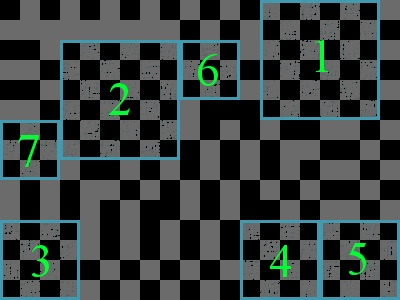
\includegraphics[width=10cm,natwidth=400,natheight=300]{image.jpg}
\end{center}

Вам дано описание листа коры шахматного дерева. Посчитайте, сколько и каких досок получится из него в конце процесса.

\InputFile
Первая строка ввода содержит количество тестов $t$. Далее следуют описания $t$ тестов. Каждый тест начинается со строки, содержащей размеры коры сетки, $m$ и $n$, при этом $n$ всегда кратна 4. Следующие $m$ строк содержат строки по $n/4$ символов --- представления строк коры в шестнадцатеричном виде. Двоичное представление этих чисел даст вам строки из $n$ бит, по одному для каждой строки. Нули обозначают черные квадраты, а единицы --- белые квадраты. Строки заданы сверху вниз. В каждой строке, наиболее значимый бит  шестнадцатеричного числа соответствует крайней слева ячейке этой строки.

Ограничения: $1\le t\le 100$, $n$ делится на 4.

В задаче 1: $1\le n, m\le 32$.

В задаче 2: $1\le n, m\le 512$.


\OutputFile
Для каждого теста выведите строку, содержащую число $k$ --- число различных размеров шахматной досок, которые будут вырезаны, следуя процедуре, описанной выше. Следующие $k$ строк должны содержать по два целых числа --- размер шахматной доски (от большего к меньшему) и количество шахматных досок такого размера, которые будут вырезаны.

\Examples

\begin{example}
\exmp{4
15 20
55555
FFAAA
2AAD5
D552A
2AAD5
D542A
4AD4D
B52B2
52AAD
AD552
AA52D
AAAAA
5AA55
A55AA
5AA55
4 4
0
0
0
0
4 4
3
3
C
C
4 4
6
9
9
6
}{5
6 2
4 3
3 7
2 15
1 57
1
1 16
2
2 1
1 12
1
2 4
}%
\end{example}

\end{problem}
